\begin{figure}
    \begin{center}
    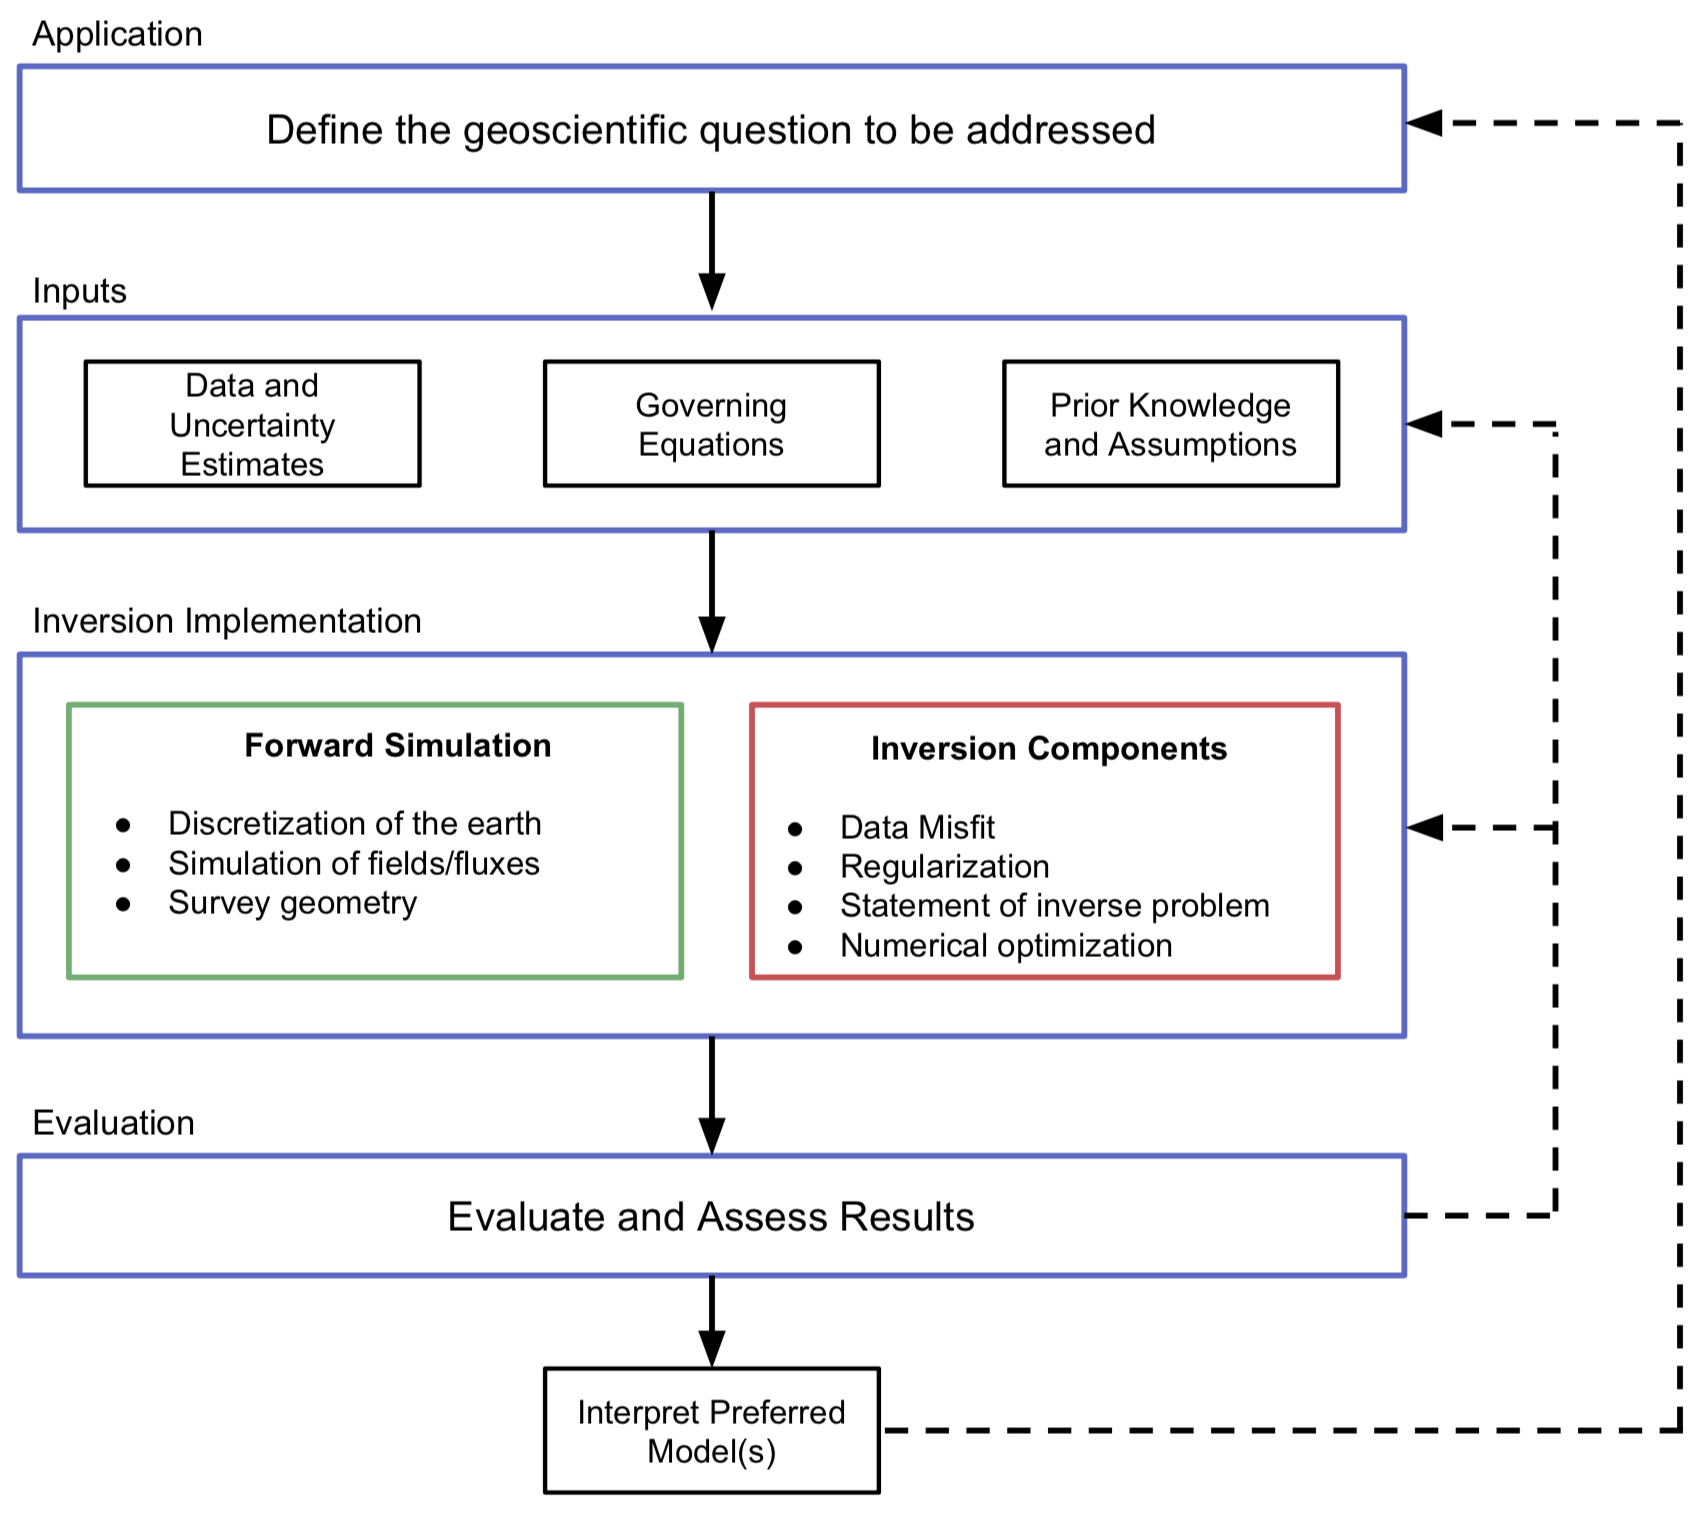
\includegraphics[width=0.8\columnwidth]{figures/InversionWorkflowBullets.png}
    \end{center}
\caption{
    Components that must be assembled to use inversion to address a geoscientific question.
    The application motivates the data-collection strategy and necessary a-priori information.
    The inversion implementation includes forward simulation components such as the discretization
    as well as inversion components such as optimization.
    Obtaining a suitable model from the inversion is an iterative process
    that requires assumptions and choices (e.g. choice of the regularization functional) be tested and re-evaluated within the context of the
    initial geoscientific question.
    Adapted from \cite{Cockett2015}.
}
\label{fig:InversionWorkflowBullets}
\end{figure}
